\documentclass[12pt, a4paper, oneside, titlepage]{report}

\usepackage{ngerman}
\usepackage[utf8]{inputenc}
\usepackage[T1]{fontenc}
\usepackage{latexsym}
\usepackage{amsmath,amsfonts,amssymb,amsthm,amscd}
\usepackage{dsfont}
\usepackage{graphicx}
\usepackage[flushleft]{paralist} 
\usepackage[dvipsnames]{xcolor} 
\usepackage[all]{xy}
\usepackage{makeidx}
\usepackage{graphicx}
\usepackage{verbatim}
\usepackage[numbers]{natbib} % [numbers,round]

\usepackage{pgf}
\usepackage{tikz}
\usepackage{pgfplots}
\usepackage{mathrsfs}
\usepackage{adjustbox}

\usetikzlibrary{arrows}
\pgfplotsset{compat=1.15}

\usepackage{hyperref}

\newcommand{\R}{\mathds{R}}
\newcommand{\Z}{\mathds{Z}}
\newcommand{\N}{\mathds{N}}
\newcommand{\Q}{\mathds{Q}}
\newcommand{\K}{\mathds{K}}
\newcommand{\C}{\mathds{C}}
\newcommand{\B}{\mathds{B}}
\newcommand{\F}{\mathds{F}}
\newcommand{\p}{\mathfrak{p}}
\newcommand{\Pot}{\mathcal{P}}
\newcommand{\id}{\textup{id}}
\newcommand{\Ker}{\textup{Ker}}
\newcommand{\Image}{\textup{Im}}
\newcommand{\la}{\langle}
\newcommand{\ra}{\rangle}

\newtheorem{lemma}{Lemma}[section]
\newtheorem{prop}[lemma]{Proposition}
\newtheorem{defprop}[lemma]{Definition and Proposition}
\newtheorem{satz}[lemma]{Satz}
\newtheorem{thm}[lemma]{Theorem} 
\newtheorem{kor}[lemma]{Korollar} 
\newtheorem{folg}[lemma]{Folgerung}
\newtheorem{verm}[lemma]{Vermutung}
\newenvironment{bew}{\begin{proof}[Beweis]}{\end{proof}}
\theoremstyle{definition} 
\newtheorem{def1}[lemma]{Definition} 
\newtheorem{bem}[lemma]{Bemerkung}
\newtheorem{bsp}[lemma]{Beispiel}
\newtheorem{notation}[lemma]{Notation}

\renewcommand\thesection{\arabic{section}}

\author{Henning Hontheim}
\title{Secret Sharing}
\date{10. März 2020}

\begin{document}
	\maketitle
	\tableofcontents
	% \clearpage
	
	\section{Wozu Secret Sharing?} % TODO
	In Public-Key-Infrastrukturen ist es oft nützlich, private Schlüssel von Teilnehmern rekonstruiren zu können. Aus Sicherheitsgründen ist es aber wichtig, dass nicht ein einzelner die Möglichkeit hat, geheime Schlüssel zu rekonstruiren. Eine Technik, um dieses Problem zu lösen, ist das Secret-Sharing, das in diesem Vortrag vorgestellt werden soll.
	\\\\
	In Public-Key-Infrastrukturen ist es oft nützlich, private Schlüssel von Teilnehmern re- konstruieren zu können. Wenn nämlich ein Benutzer die Chipkarte mit seinem geheimen Schlüssel verliert, kann er seine verschlüsselt gespeicherten Daten nicht mehr entschlüsseln. Aus Sicherheitsgründen ist es aber wichtig, dass nicht ein einzelner die Möglichkeit hat, geheime Schlüssel zu rekonstruieren. Es ist besser, wenn bei der Rekonstruktion von privaten Schlüsseln mehrere Personen zusammenarbeiten müssen. Die können sich dann gegenseitig kontrollieren. Die Wahrscheinlichkeit sinkt, dass Unberechtigte Zugang zu geheimen Schlüsseln bekommen. In diesem Kapitel wird eine Technik vorgestellt, dieses Problem zu lösen, das Secret-Sharing. \cite{buchmann} \cite{shamir}
	
	\subsection{Ein kombinatorisches Beispiel}
	
	Mehrere Wissenschaftler $ N $ arbeiten zusammen an einem Geheimprojekt. Um die Dokumente geheim zu halten und um Missbrauch vorzubeugen, verschließen sie diese in einem Tresor. Nur wenn mindestens die Hälfte aller Wissenschaftler anwesend ist, soll sich der Tresor öffnen lassen. Wie viele paarweise verschiedene Schlösser $ S $ muss der Tresor mindestens besitzen? Wie viele paarweise verschiedene Schlüssel $ s $ muss jeder Wissenschaftler mindestens bei sich tragen? Siehe \cite{shamir} nach \cite{liu}.
	
	\begin{bsp}
		Sei $ N = 11 $ die Anzahl aller Wissenschaftler und $ n = \left\lceil\frac{N}{2} \right\rceil = 6 $ die Anzahl derer, die mindestens anwesend sein müssen, damit sich der Tresor öffnen lässt. Folglich muss es also für jede Teilmenge mit $ k $ Wissenschaftlern, wobei $ k = N - n = 5 $, genau ein Schloss geben, für das keiner der $ k $ Wissenschaftler einen Schlüssel besitzt. Also muss der Tresor $ S = \binom{N}{k} = \binom{11}{5} = 462 $ paarweise verschiedene Schlösser besitzen.
		
		Sei $ W = \{w_1, w_2, \dots w_k, w_{k+1}\} $ mit $ |W| = k + 1 = 6 $ die Menge von Wissenschaftlern, die mindestens benötigt wird, um den Tresor zu öffnen. Dann gibt es genau ein bestimmtes Schloss $ S' $, für das keiner der Wissenschaftler aus $ W \setminus w_{k+1} $ einen Schlüssel besitzt, der Wissenschaftler $ w_{k+1} $ jedoch schon. Da für jede Permutation von $ k = 5 $ Wissenschaftlern genau der $ w_{k+1} $ existiert, der die Teilmenge $ W $ \glqq vervollständigt\grqq, bekommt jeder Wissenschaftler $ s = \binom{N-1}{|W|-1} = \binom{N-1}{k} = \binom{10}{5} = 252 $ Schlüssel. Das ergibt eine Gesamtanzahl an $ 11 \cdot 252 = 2772 $ Schlüsseln. Dass dies keine praktikable Lösung des Problems ist, ist offensichtlich.
	\end{bsp}
	
	\section{Primitives Secret Sharing}
	\subsection{Aufsplitten des Secrets}
		Blah % TODO
		
		\begin{bsp}
			Zahl aufteilen % TODO
		\end{bsp}
		
	\subsection{One-Time-Padding}
		 Blah % TODO
		 
	\begin{bsp}
		Zwei Personen % TODO
	\end{bsp}

	\begin{bsp}
		$ n $ Personen % TODO
	\end{bsp}

	\begin{bsp}
		Visuelles Beispiel % TODO
	\end{bsp}
	
	\section{Shamir's Secret Sharing}
		Blah % TODO
		
	\subsection{$ (2,n) $-Schema}
		Blah % TODO
		
		\begin{figure}[h]
		\begin{adjustbox}{center}
			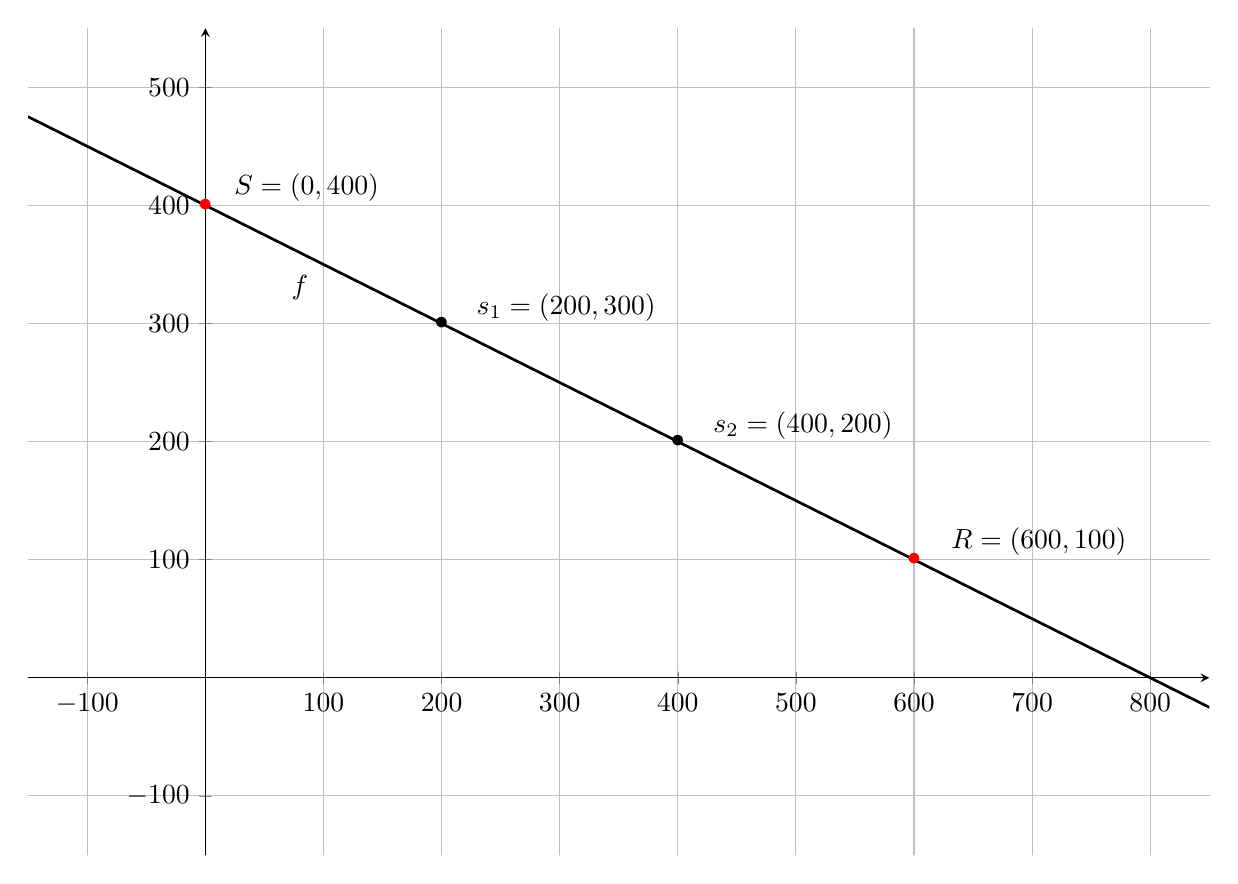
\begin{tikzpicture}[line cap=round,line join=round,>=triangle 45,x=0.015cm,y=0.015cm]
				\begin{axis}[x=0.015cm,y=0.015cm,axis lines=middle,ymajorgrids=true,xmajorgrids=true,
				xmin=-150.,xmax=850.,xtick={-100.,0.,...,850.},
				ymin=-150.,ymax=550.,ytick={-100.,0.,...,550.},]
				\clip(-150.,-150.) rectangle (850.,550.);
				\draw [line width=1.pt,domain=-150.:850.] plot(\x,{(--240000.-300.*\x)/600.});
				\draw (80.,330.) node {$f$};
				\draw[color=red] (0.,400.) node {$ \bullet $};
				\draw (85.724885311689992,414.69861484203665) node {$S=(0,400)$};
				\draw[color=red] (600.,100.) node {$ \bullet $};
				\draw (705.7349442961975,115.09627666453882) node {$R=(600,100)$};
				\draw (200.,300.) node {$ \bullet $};
				\draw (305.45977743002265,313.2204035238519) node {$s_1=(200,300)$};
				\draw (400.,200.) node {$ \bullet $};
				\draw (506.0000521778647,213.35295746468594) node {$s_2=(400,200)$};
				\end{axis}
			\end{tikzpicture}
		\end{adjustbox}
		\caption{Erweiterung des Geheimnisses $ S $ als Gerade $ f $ für zwei Shares $s_1$ und $s_2$.} % TODO
	\end{figure}

	\subsection{$ (3,n) $-Schema}
		Blah % TODO
		
	\begin{figure}[h]
		\begin{adjustbox}{center}
			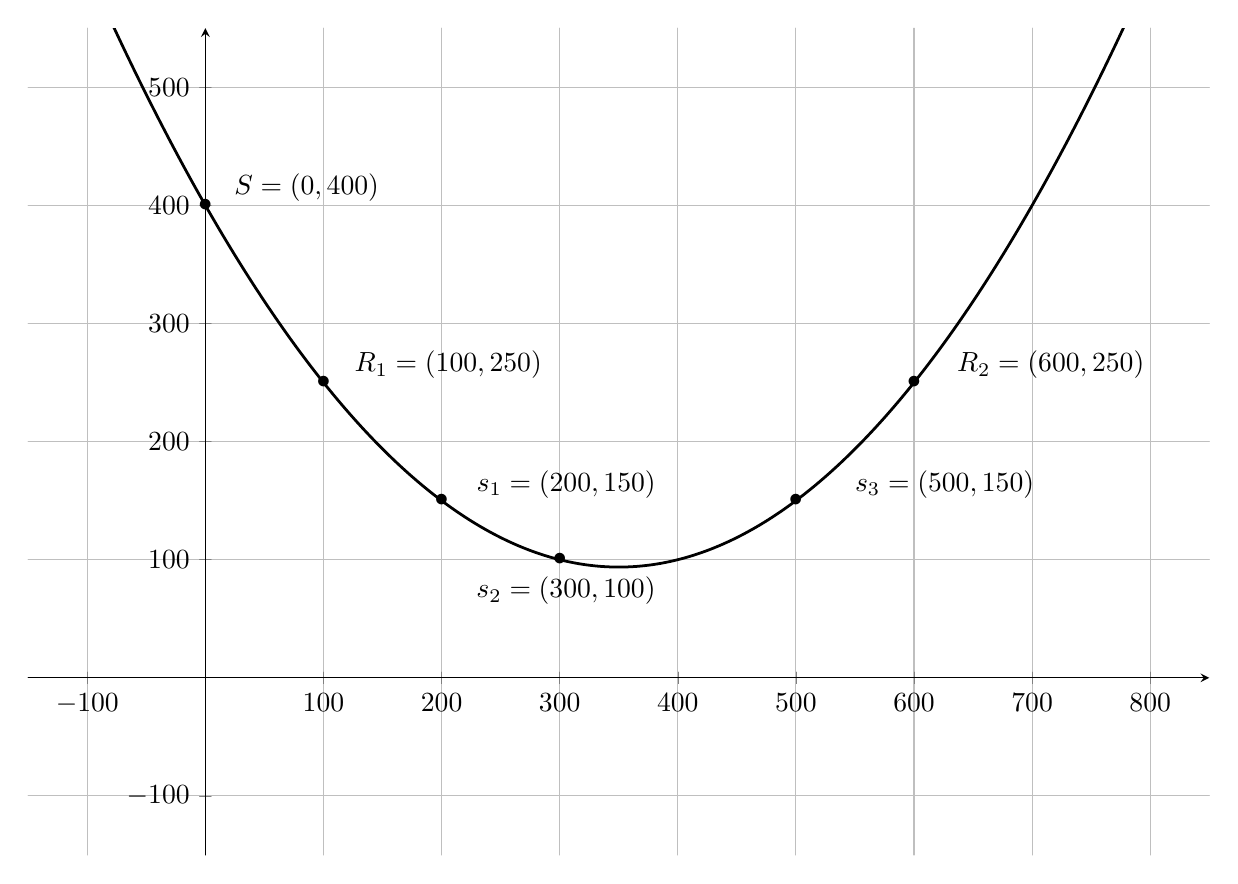
\begin{tikzpicture}[line cap=round,line join=round,>=triangle 45,x=0.015cm,y=0.015cm]
			\begin{axis}[x=0.015cm,y=0.015cm,axis lines=middle,ymajorgrids=true,xmajorgrids=true,
			xmin=-150.,xmax=850.,xtick={-100.,0.,...,850.},
			ymin=-150.,ymax=550.,ytick={-100.,0.,...,550.},]
			\clip(-150.,-150.) rectangle (850.,550.);
			\draw[line width=1.pt,smooth,samples=100,domain=-150.0:850.0] plot(\x,{0.0025*(\x)^(2.0)-1.75*(\x)+400.0});
			\draw (0.,400.) node {$ \bullet $};
			\draw (85.724885311689992,414.69861484203676) node {$S=(0,400)$};
			\draw (100.,250.) node {$ \bullet $};
			\draw (205.59233137085631,264.8974457532878) node {$R_1=(100,250)$};
			\draw (600.,250.) node {$ \bullet $};
			\draw (715.7349442961975,264.8974457532878) node {$R_2=(600,250)$};
			\draw (488.95446301733347,566.9159318193139) node {$f$};
			\draw (200.,150.) node {$ \bullet $};
			\draw (305.45977743002265,163.41923443510308) node {$s_1=(200,150)$};
			\draw (300.,100.) node {$ \bullet $};
			\draw (305.32722348918895,73.4855114055201) node {$s_2=(300,100)$};
			\draw (500.,150.) node {$ \bullet $};
			\draw (625.86749823703104,163.41923443510308) node {$s_3=(500,150)$};
			\end{axis}
			\end{tikzpicture}
		\end{adjustbox}
		\caption{Parabel} % TODO
	\end{figure}

	\subsection{Allgemeine $ (k,n) $-Schemata}
		Blah % TODO
	
	\subsection{Shamir's Secret Sharing $ x \bmod p $}
		Blah % TODO

	\section{Weitere Verfahren}
		Blah % TODO
		
	\subsection{Blakeley's}
		Blah % TODO
		
	\subsection{whatever\dots}
		Blah % TODO
	
	\section{Fazit}
	
	\cleardoublepage
	\phantomsection
	\addcontentsline{toc}{chapter}{Abbildungsverzeichnis}
	\listoffigures
	\begingroup
	\let\clearpage\relax
	\phantomsection
	\addcontentsline{toc}{chapter}{Literaturverzeichnis}
	\bibliographystyle{acm} % siam, alpha, alphadin, ieeetr, plain, acm, abbrvdin
	\bibliography{secret-sharing}
	\endgroup
\end{document}
